% The orbit-stabilizer bijection: cosets gS of the stabilizer S ⊆ G
% correspond to points of the orbit O ⊆ X, via g ↦ g·x.
% Source: book/tex/H113/action.tex (§ Orbits and stabilizers).
\documentclass[border=2mm]{standalone}
\usepackage{tikz}
\usetikzlibrary{arrows.meta}
\begin{document}
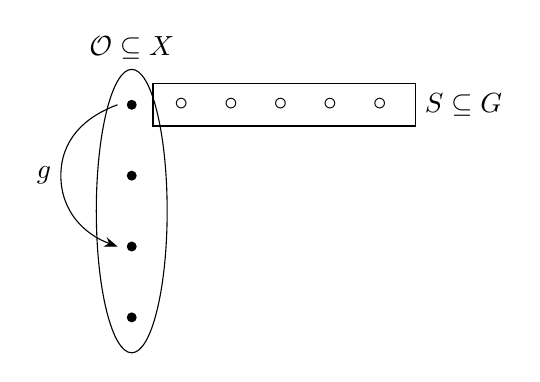
\begin{tikzpicture}[scale=0.9]
  % The orbit O inside X.
  \draw (0,0) ellipse (0.5 and 2);
  \node[above] at (0,2) {$\mathcal O \subseteq X$};
  \foreach \i in {-1.5,-0.5,0.5,1.5} \fill (0,\i) circle (2pt);
  % The stabilizer S inside G.
  \draw (0.3,1.2) rectangle (4,1.8);
  \node[right] at (4,1.5) {$S \subseteq G$};
  \foreach \i in {0.7,1.4,2.1,2.8,3.5} \node at (\i,1.5) {$\circ$};
  % The map g.
  \draw[-{Stealth}] (-0.2,1.5) to[out=200,in=90] (-1,0.5) to[out=-90,in=160] (-0.2,-0.5);
  \node[left] at (-1,0.5) {$g$};
\end{tikzpicture}
\end{document}
